
\documentclass[a4paper,11pt]{article}
\usepackage[a4paper, margin=8em]{geometry}

% usa i pacchetti per la scrittura in italiano
\usepackage[french,italian]{babel}
\usepackage[T1]{fontenc}
\usepackage[utf8]{inputenc}
\frenchspacing 

% usa i pacchetti per la formattazione matematica
\usepackage{amsmath, amssymb, amsthm, amsfonts}

% usa altri pacchetti
\usepackage{gensymb}
\usepackage{hyperref}
\usepackage{standalone}

% imposta il titolo
\title{Appunti Calcolo Numerico}
\author{Luca Seggiani}
\date{2025}

% disegni
\usepackage{pgfplots}
\pgfplotsset{width=10cm,compat=1.9}

% imposta lo stile
% usa helvetica
\usepackage[scaled]{helvet}
% usa palatino
\usepackage{palatino}
% usa un font monospazio guardabile
\usepackage{lmodern}

% tikz in sans
\tikzset{every picture/.style={/utils/exec={\sffamily}}}

\renewcommand{\rmdefault}{ppl}
\renewcommand{\sfdefault}{phv}
\renewcommand{\ttdefault}{lmtt}

% circuiti
\usepackage{circuitikz}
\usetikzlibrary{babel}

% disponi il titolo
\makeatletter
\renewcommand{\maketitle} {
	\begin{center} 
		\begin{minipage}[t]{.8\textwidth}
			\textsf{\huge\bfseries \@title} 
		\end{minipage}%
		\begin{minipage}[t]{.2\textwidth}
			\raggedleft \vspace{-1.65em}
			\textsf{\small \@author} \vfill
			\textsf{\small \@date}
		\end{minipage}
		\par
	\end{center}

	\thispagestyle{empty}
	\pagestyle{fancy}
}
\makeatother

% disponi teoremi
\usepackage{tcolorbox}
\newtcolorbox[auto counter, number within=section]{theorem}[2][]{%
	colback=blue!10, 
	colframe=blue!40!black, 
	sharp corners=northwest,
	fonttitle=\sffamily\bfseries, 
	title=Teorema~\thetcbcounter: #2, 
	#1
}

% disponi definizioni
\newtcolorbox[auto counter, number within=section]{definition}[2][]{%
	colback=red!10,
	colframe=red!40!black,
	sharp corners=northwest,
	fonttitle=\sffamily\bfseries,
	title=Definizione~\thetcbcounter: #2,
	#1
}

% disponi problemi
\newtcolorbox[auto counter, number within=section]{problem}[2][]{%
	colback=green!10,
	colframe=green!40!black,
	sharp corners=northwest,
	fonttitle=\sffamily\bfseries,
	title=Problema~\thetcbcounter: #2,
	#1
}

% disponi codice
\usepackage{listings}
\usepackage[table]{xcolor}

\definecolor{codegreen}{rgb}{0,0.6,0}
\definecolor{codegray}{rgb}{0.5,0.5,0.5}
\definecolor{codepurple}{rgb}{0.58,0,0.82}
\definecolor{backcolour}{rgb}{0.95,0.95,0.92}

\lstdefinestyle{codestyle}{
		backgroundcolor=\color{black!5}, 
		commentstyle=\color{codegreen},
		keywordstyle=\bfseries\color{magenta},
		numberstyle=\sffamily\tiny\color{black!60},
		stringstyle=\color{green!50!black},
		basicstyle=\ttfamily\footnotesize,
		breakatwhitespace=false,         
		breaklines=true,                 
		captionpos=b,                    
		keepspaces=true,                 
		numbers=left,                    
		numbersep=5pt,                  
		showspaces=false,                
		showstringspaces=false,
		showtabs=false,                  
		tabsize=2
}

\lstdefinestyle{shellstyle}{
		backgroundcolor=\color{black!5}, 
		basicstyle=\ttfamily\footnotesize\color{black}, 
		commentstyle=\color{black}, 
		keywordstyle=\color{black},
		numberstyle=\color{black!5},
		stringstyle=\color{black}, 
		showspaces=false,
		showstringspaces=false, 
		showtabs=false, 
		tabsize=2, 
		numbers=none, 
		breaklines=true
}

\lstdefinelanguage{javascript}{
	keywords={typeof, new, true, false, catch, function, return, null, catch, switch, var, if, in, while, do, else, case, break},
	keywordstyle=\color{blue}\bfseries,
	ndkeywords={class, export, boolean, throw, implements, import, this},
	ndkeywordstyle=\color{darkgray}\bfseries,
	identifierstyle=\color{black},
	sensitive=false,
	comment=[l]{//},
	morecomment=[s]{/*}{*/},
	commentstyle=\color{purple}\ttfamily,
	stringstyle=\color{red}\ttfamily,
	morestring=[b]',
	morestring=[b]"
}

% disponi sezioni
\usepackage{titlesec}

\titleformat{\section}
	{\sffamily\Large\bfseries} 
	{\thesection}{1em}{} 
\titleformat{\subsection}
	{\sffamily\large\bfseries}   
	{\thesubsection}{1em}{} 
\titleformat{\subsubsection}
	{\sffamily\normalsize\bfseries} 
	{\thesubsubsection}{1em}{}

% disponi alberi
\usepackage{forest}

\forestset{
	rectstyle/.style={
		for tree={rectangle,draw,font=\large\sffamily}
	},
	roundstyle/.style={
		for tree={circle,draw,font=\large}
	}
}

% disponi algoritmi
\usepackage{algorithm}
\usepackage{algorithmic}
\makeatletter
\renewcommand{\ALG@name}{Algoritmo}
\makeatother

% disponi numeri di pagina
\usepackage{fancyhdr}
\fancyhf{} 
\fancyfoot[L]{\sffamily{\thepage}}

\makeatletter
\fancyhead[L]{\raisebox{1ex}[0pt][0pt]{\sffamily{\@title \ \@date}}} 
\fancyhead[R]{\raisebox{1ex}[0pt][0pt]{\sffamily{\@author}}}
\makeatother

\begin{document}

% sezione (data)
\section{Lezione del 28-04-25}

% stili pagina
\thispagestyle{empty}
\pagestyle{fancy}

% testo
\subsection{Approssimazione di integrali}
Vorremo quindi approssimare funzioni del tipo:
$$
I(\rho \cdot f) = \int_a^b f(x) \cdot \rho(x) \, dx
$$
dove $f: [a, b] \rightarrow \mathbb{R}$ continua $\in C\left([a, b]\right)$, mentre $\rho(x) : [a, b] \rightarrow \mathbb{R}$ sempre continua $\in C\left([a, b]\right)$ è una funzione particolare, spesso la funzione unitaria o comunque una funzione detta \textbf{funzione peso} tale che:
\begin{itemize}
	\item $\rho(x)$ è positiva:
		$$ \rho(x) \geq 0 $$
	\item $\rho(x)$ rispetta le condizioni:
		$$ m_k = \int_a^b x^k \rho(x) \, dx < +\infty, \quad \forall k = 0, 1, ... $$
\end{itemize}

Veniamo alle motivazioni dell'approssimazione di integrali. 
Potremmo voler approssimare integrali del tipo:
$$
\int_a^b f(x) \, dx \quad \left( \rho(x) = 1 \right)
$$
per una serie di motivi:
\begin{itemize}
	\item Di molte funzioni non si può trovare un'espressione semplice della primitiva di $f$ (funzioni ellittiche, funzioni su più variabili, ecc...);
	\item Anche se esiste la primitiva potrebbe essere particolarmente oneroso in termini di risorse computazioniali calcolarla o valutarla in un punto per ottenere l'integrale;
	\item Come nel caso dell'approssimazione e dell'interpolazione, ci sono casi in cui della $f$ si conoscono solo alcuni punti, cioè non se ne ha un'espressione esplicita che possiamo integrare. Vedremo che sarà questo il caso più comune.
\end{itemize}

Prendiamo quindi il caso dove conosciamo una serie di punti $(x_i, f(x_i))$ di $f(x)$.
L'idea per approssimare l'integrale sarà di considerare una formula del tipo:
$$
\int_a^b f(x) \rho(x) \, dx \approx \sum_{i = 0}^n f(x_i) \cdot a_i
$$
con:
$$
a \leq x_0 < x_1 < ... < x_n \leq b
$$
In questo caso chiamiamo gli $x_i$ \textbf{nodi} e gli $a_i$ \textbf{pesi}, e la formula \textbf{formula di quadratura}.
Si ha quindi che una formula di quadratura è univocamente determinata una volta decisi nodi e pesi.

Definiamo quindi formalmente:
\begin{definition}{Formula di quadratura}
	Dati un intervallo $[a, b]$ e $\rho(x)$, definiamo $J_n(\circ)$ formula di quadratura su $(n + 1)$ nodi $x_0, ..., x_n$ con pesi $a_0, ..., a_n$ la funzione:
	\begin{itemize}
		\item Di questa forma:
	$$
	J_n : C\left([a, b]\right) \rightarrow \mathbb{R}
	$$
	tale che:
	$$
	f \rightarrow \sum_{i=0}^n f(x_i) \cdot a_i
	$$
		\item
	O equivalentemente:
	$$
	J_n : \mathbb{R}^{n + 1} \rightarrow \mathbb{R}
	$$
	tale che:
	$$
	\begin{pmatrix}
		f_0 \\ \vdots \\ f_n
	\end{pmatrix} 
	\rightarrow
	\sum_{i=0}^n f_i \cdot a_i
	$$
	\end{itemize}
\end{definition}

\noindent
\begin{minipage}{\textwidth}
Data la definizione di formula di quadratura, possiamo quindi definire l'errore:
\begin{definition}{Errore della formula di quadratura}
	L'errore della formula di quadratura $J_n(\circ)$ si definisce come:
	$$
	E_n(f) = \int_a^b f(x) \rho(x) \, dx - J_n(f) = \int_a^b f(x) \rho(x) \, dx - \sum_{i = 0}^n f(x_i) \cdot a_i
	$$
	anche questa tale che:
	$$
	E_n : C\left([a, b]\right) \rightarrow \mathbb{R}
	$$
	con:
	$$
	f \rightarrow E_n(f)
	$$
\end{definition}
\end{minipage}

Ossserviamo che sia $J_n$ che $E_n$ sono funzioni lineari, in quanto date $f_1, f_2 \in C\left([a, b]\right)$ e $c_1, c_2 \in \mathbb{R}$:
$$
J_n (c_1 f_1 + c_2 f_2) = \sum_{i = 0}^n a_i (c_1 f_1 + c_2 f_2)(x_i) 
= \sum_{i = 0}^n a_i ( c_1 f_1(x_i) + c_2 f_2(x_i) )
$$
$$
= \sum_{i = 0}^n \left( a_i c_1 f_1 (x_i) + a_i c_2 f_2 (x_i) \right)
= c_1 \sum_{i = 0}^n a_i f_1 (x_i) + c_2 \sum_{i = 0}^n a_i f_2 (x_i)
= c_1 J_n(f_1) + c_2 J_n(f_2)
$$
e analogamente con $E_n$. \qed

Potremmo quindi chiederci quando una formula di quadratura è accurata.
Potremmo definire un primo indicatore detto \textbf{grado di precisione}.
\begin{definition}{Grado di precisione}
	Data $J_n$ formula di quadratura definiamo grado di precisione (a volte detto \textit{grado di precisione algebrico}) il naturale $m \in \mathbb{N}$ tale che:
	$$
		E_n(1) = E_n(x) = ... = E_n (x^m) = 0
	$$
	presi i monomi $x_0, ..., x^m$, cioè per cui:
	$$
	E_n(x^{m + 1}) \neq 0
	$$
\end{definition}

Osserviamo che per la proprietà di linearità di $E_n$ e $J_n$ appena dimostrata, si ha che $J_n$ ha grado di precisione $m$ se e solo se $J_n$ integra esattamente tutti i polinomi di grado $\leq m$ (che altro non sono che combinazioni lineari dei monomi $x_0, ..., x^{m}$ appena considerati).

\subsubsection{Formula dei trapezi}

Prendiamo ad esempio $\rho = 1$, l'intervallo $[a, b] = [-1, 1]$ con $n = 1$, per cui consideriamo solo gli estremi $x_0 = -1$, $x_1 = 1$.
In questo caso avremo la formula di quadratura:
$$
J_1 (f) = a_0 f(-1) + a_1 f(1) \approx \int_{-1}^{1} f(x) \, dx
$$

Potremmo chiederci qual'è la migliore scelta dei coefficienti di peso $a_i$.
Questi saranno chiaramente quelli che massimizzano il grado di precisione $m$ della formula di quadratura $J_m$.
Vorremmo quindi imporre due condizioni:
$$
	\begin{cases}
		E_n(1) = 0 \\
		E_n(x) = 0
	\end{cases}
	\rightarrow
	\begin{cases}
		\int_{-1}^1 1 \, dx - (a_0 + a_1) = 0 \\
		\int_{-1}^1 x \, dx - (-a_0 + a_1) = 0
	\end{cases}
	\rightarrow
	\begin{cases}
		2 - a_0 - a_1 = 0 \\
		0 + a_0 - a_1 = 0
	\end{cases}
$$i
da cui risolvendo il sistema si ha:
$$a_0, a_1 = 1$$

Il risultato sarà quindi che la formula di quadratura è:
$$
J_1 (f) = f(-1) + f(1)
$$
con grado di precisione almeno 1 ($m \geq 1$).

Verifichiamo infatti cosa accade per gradi $> m$, ad esempio grado 2:
$$
E_n(x^2) = \int_{-1}^1 x^2 \, dx - (1 + 1) = \frac{2}{3} - 2 \neq 0
$$
per cui $m$ è esattamente 1.

Graficamente, questo non significherà altro che approssimare l'integrale fra $-1$ e $1$ attraverso l'area sottesa alla retta passante per i punti $(-1, f(-1))$, $(1, f(1))$, cosa che chiaramente risulta inadeguata quando $f$ è di grado maggiore a 1 (come ad esempio una parabola).
Vediamo infatti su un grafico che dato $a$ e $b$ consideriamo l'area evidenziata in viola:
\begin{center}
	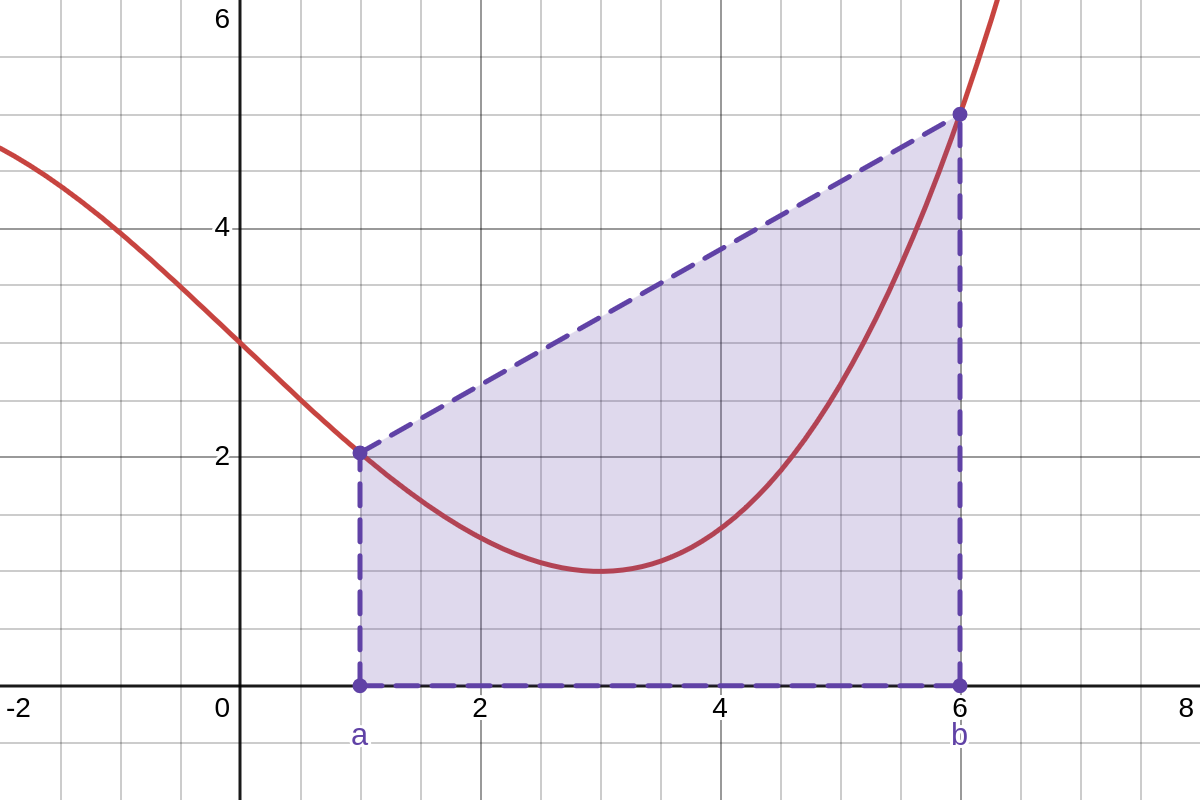
\includegraphics[scale=0.28]{../figures/trapezoidal_approx.png}
\end{center}

Quest'area è effettivamente un trapezio, motivo per cui la formula $J_1$ sul generico intervallo $[a, b]$ viene detta \textbf{formula dei trapezi}:
$$
\left(f(a) + f(b)\right) \frac{b - a}{2}
$$
Possiamo dimostrare questa in 2 modi:
\begin{itemize}
	\item Applicando direttamente l'area del trapezio, cioè:
		$$
		(b + B) \frac{h}{2} = \left(f(a) + f(b)\right) \frac{b - a}{2}
		$$ \qed
	\item Alternativamente possiamo ricorrere all'imposizione di un sistema simile a quello visto prima all'intervallo generico $[a, b]$:
\[
	\begin{cases}
		E_n(1) = 0 \\ 
		E_n(x) = 0
	\end{cases}
	\rightarrow
	\begin{cases}
		\int_a^b 1 \, dx - a_0 - a_1 = 0 \\ 
		\int_a^b x \, dx - a \cdot a_0 - b \cdot a_1 = 0
	\end{cases}
\]
\[
	\rightarrow
	\begin{cases}
		b - a = a_0 + a_1 \\ 
		\frac{x^2}{2} \Big|^b_a = a \cdot a_0 + b \cdot a_1 
	\end{cases}
	\rightarrow
	\begin{cases}
		b - a = a_0 + a_1 \\ 
		\frac{b^2}{2} - \frac{a^2}{2} = a \cdot a_0 + b \cdot a_1 
	\end{cases}
\]
da cui si ottiene il sistema:
\[
	\begin{cases}
		a_0 + a_1 = b - a \\ 
		a \cdot a_0 + b \cdot a_1 = \frac{b^2 - a^2}{2}
	\end{cases}
\]
Prendiamo ad esempio $a_0$ dalla prima equazione:
$$
a_0 = b - a - a_1
$$
che sostituendo nella seconda equazione dà:
$$
a(b - a - a_1) + b a_1 = \frac{b^2 - a^2}{2} \, \Rightarrow \, ab - a^2 - aa_1 + ba_1 = \frac{b^2 - a^2}{2}
$$
$$
\implies (b - a) a_1 = \frac{b^2 - a^2}{2} - ab + a^2 = \frac{a^2 - 2ab + b^2}{2} = \frac{(b - a)^2}{2}
$$
dove guardando gli estremi si ha:
$$
a_1 = \frac{b - a}{2}
$$
Dalla prima equazione, poi, è immediato che anche:
$$
a_0 = \frac{b - a}{2}
$$
da cui la formula dei trapezi. \qed
\end{itemize}

\subsubsection{Formula di Simpson}

Vediamo di raffinare la formula dei trapezi aggiungendo un nodo in più, ad esempio il punto intermedio fra gli estremi dell'intervallo $[a, b]$.
Nel caso $[-1, 1]$, questo non sarà altro che $0$, per cui $x_0 = -1$, $x_1 = 0$, $x_2 = 1$.
Avremo che la formula di quadratura è:
$$
J_2 (f) = a_0 f(-1) + a_1 f(0) + a_2 f(1)
$$
e scegliamo gli $a_0, a_1, a_2 \in \mathbb{R}$ per massimizzare il grado di precisione, con procedimento analogo a prima:
$$
	\begin{cases}
		E_n(1) = 0 \\	
		E_n(x) = 0 \\	
		E_n(x^2) = 0	
	\end{cases}
	\rightarrow
	\begin{cases}
		2 = a_0 + a_1 + a_2 \\
		0 = -a_0 + a_2 \\
		\frac{2}{3} = a_0 + a_2
	\end{cases}
$$
da cui:
$$
a_0 = a_2 = \frac{1}{3}, \quad a_1 = \frac{4}{3}
$$

Il risultato sarà quindi che la formula di quadratura è:
$$
J_2(f) = \frac{1}{3} \left( f(-1) + 4 f(0) + f(1) \right)
$$
detta anche \textbf{formula di Simpson} o di \textit{Cavalieri-Simpson}.

Vediamo cosa succede per l'integrale del monomio di grado 3 attraverso la formula di Simpson:
$$
E_2 (x^3) = \int_{-1}^1 x^3 \, dx - \frac{1}{3} \left( -1 + 4 \cdot 0 + 1 \right) = 0
$$
cioè abbiamo grado non solo $\geq 2$, ma anche $\geq 3$, per cui consideriamo il grado 4:
$$
E_2 (x^4) = \int_{-1}^1 x^4 \, dx - \frac{1}{3} \left( 1 + 4 \cdot 0 + 1 \right) = \frac{2}{5} - \frac{2}{3} \neq 0
$$
per cui abbiamo che il grado di precisione della formula di Simpson è esattamente $m = 3$.

\par\smallskip

Infine generalizziamo la formula di Simspon all'intervallo $[a, b]$:
$$
\frac{b - a}{6} \left( f(a) + 4 f\left( \frac{a + b}{2} \right) + f(b) \right)
$$
Questa si dimostra per calcolo diretto, imponendo le condizioni sul generico intervallo $[a, b]$:
\[
	\begin{cases}
		E_n(1) = 0 \\ 
		E_n(x) = 0 \\ 
		E_n(x^2) = 0
	\end{cases}
	\rightarrow
	\begin{cases}
		\int_a^b 1 \, dx - a_0 - a_1 - a_2 = 0 \\ 
		\int_a^b x \, dx - a \cdot a_0 - \frac{a + b}{2} a_1 - b \cdot a_2 = 0 \\ 
		\int_a^b x^2 \, dx - a^2 \cdot a_0 - \frac{(a+b)^2}{4} a_1 - b^2 \cdot a_2 = 0
	\end{cases}
\]
\[
	\rightarrow 
	\begin{cases}
		b - a = a_0 + a_1 + a_2 \\ 
		\frac{b^2}{2} - \frac{a^2}{2} = a \cdot a_0 + \frac{a + b}{2} a_1 + b \cdot a_2 \\ 
		\frac{b^3}{3} - \frac{a^3}{3} = a^2 \cdot a_0 + \frac{(a + b)^2}{4} a_1 + b^2 \cdot a_2
	\end{cases}
\]
Abbiamo che dalla prima equazione si ricava:
$$
a_0 = b - a - a_1 - a_2
$$
mentre dalla seconda si ha, sostituendo:
$$
\frac{b^2 - a^2}{2} = a(b - a - a_1 - a_2) + \frac{a + b}{2} a_1 + b a_2 =
$$
$$
= ab - a^2 - a \cdot a_1 - a \cdot a_2 + \frac{a + b}{2} a_1 + b a_2
$$
$$
\implies \frac{b^2 - a^2}{2} - ab + a^2 = -a \cdot a_1 - a \cdot a_2 + \frac{a + b}{2} a_1 + b \cdot a_2
$$
$$
\Rightarrow \, \frac{b^2 - a^2 - 2ab + 2a^2}{2} = a_1 \left( -a + \frac{a + b}{2} \right) + a_2 (b - a) \, \Rightarrow \frac{(b-a)^2}{2} = a_1 \left( \frac{b - a}{2} \right) + a_2 (b - a)
$$
da cui:
$$
a_1 = b - a - 2 a_2
$$
Sostituendo questo nella formula trovata prima per $a_0$ si trova quindi:
$$
a_0 = b - a - b + a + 2 a_2 - a_2 = a_2
$$
cioè valgono le condizioni:
\[
	\begin{cases}
		a_0 = a_2 \\ 
		a_1 = b - a - 2 a_0 = b - a - 2 a_2
	\end{cases}
\]
Usiamo queste per trovare $a_0$ (o equivalentemente $a_2$) dalla terza equazione.
Avremo in questo caso:
$$
\frac{b^3}{3} - \frac{a^3}{3} = a^2 \cdot a_0 + \frac{(a + b)^2}{4} a_1 + b^2 \cdot a_0
= a^2 \cdot a_0 + \frac{(a + b)^2}{4} (b - a - 2a_0) + b^2 \cdot a_0
$$
$$
= a^2 \cdot a_0 + b^2 \cdot a_0 + \frac{(a + b)^2}{4} (b - a) - \frac{(a + b)^2}{2} a_0
$$
dove vorremo dividere i termini fra parte sinistra e destra come:
$$
\frac{b^3 - a^3}{3} - \frac{(a + b)^2}{4} (b - a) = a^2 \cdot a_0 + b^2 \cdot a_0 - \frac{(a + b)^2}{2} a_0 
$$
Valutiamo queste separatamente.
\begin{itemize}
	\item \textbf{Parte sinistra}:
		$$
		\frac{b^3 - a^3}{3} - \frac{(a + b)^2}{4} (b - a) = \frac{b^3 - a^3}{3} - \frac{a^2 + 2ab + b^2}{4} (b - a)
		$$
		$$
		= \frac{b^3 - a^3}{3} - \frac{a^2 b - a^3 + 2ab^2 - 2 a^2 b + b^3 - ab^2}{4} = \frac{b^3 - a^3}{3} + \frac{-b^3 + a^3 + a^2 b - a b^2}{4}
		$$
		$$
		= \frac{1}{12}b^3 - \frac{1}{12}a^3 + \frac{1}{4}a^2 b - \frac{1}{4} a b^2 = \frac{1}{12} (b - a)^3
		$$
		
	\item \textbf{Parte destra}:
		$$
		a^2 \cdot a_0 + b^2 \cdot a_0 - \frac{(a + b)^2}{2} a_0 = a^2 \cdot a_0 + b^2 \cdot a_0 - \left( \frac{a^2}{2} + ab + \frac{b^2}{2} \right) a_0
		$$
		$$
		= \frac{a^2}{2} a_0 + \frac{b^2}{2} a_0 - ab \cdot a_0 = \frac{(b - a)^2}{2} a_0
		$$
\end{itemize}
da cui avremo quindi complessivamente:
$$
\frac{1}{12} (b - a)^3 = \frac{(b - a)^2}{2} a_0 \implies a_0 = \frac{b - a}{6}
$$
da cui si ha immediatamente che:
$$
a_0 = a_2 = \frac{2}{3} (b - a)
$$
che dà esattamente la formula di Simpson. \qed

\par\smallskip

Abbiamo quindi che anche Simspon si basa sul trovare implicitamente il polinomio interpolante e poi integrare quello, con la caratteristica aggiunta che anche al grado 3 l'integrale risulta esatto (anche se non lo è l'interpolante).
In particolare, vediamo sul grafico che l'interpolante per una quadratica da il risultato esatto:
\begin{center}
	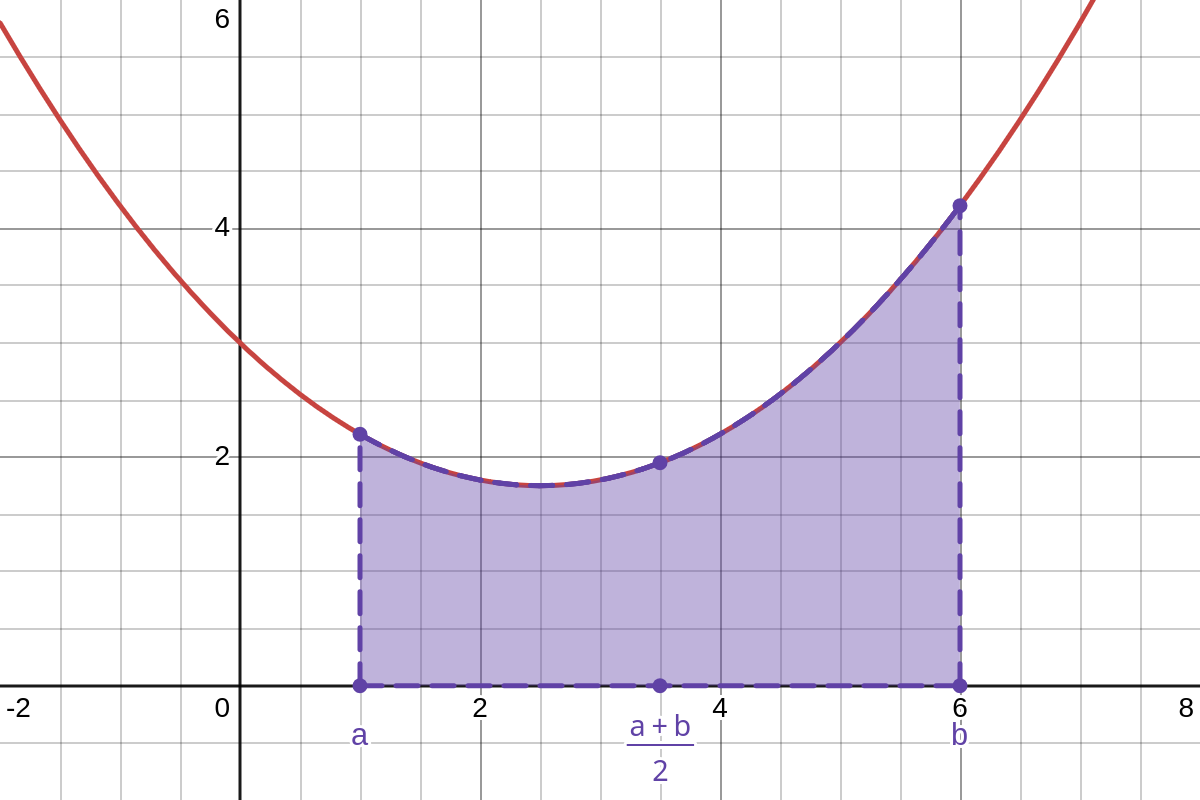
\includegraphics[scale=0.28]{../figures/simpson_quadratic.png}
\end{center}
e che per una cubica, anche se l'interpolante non coincide con la funzione, si ha comunque risultato esatto.
Questo è dato dal fatto che si creano due regioni discordi che si compensano fra di loro:
\begin{center}
	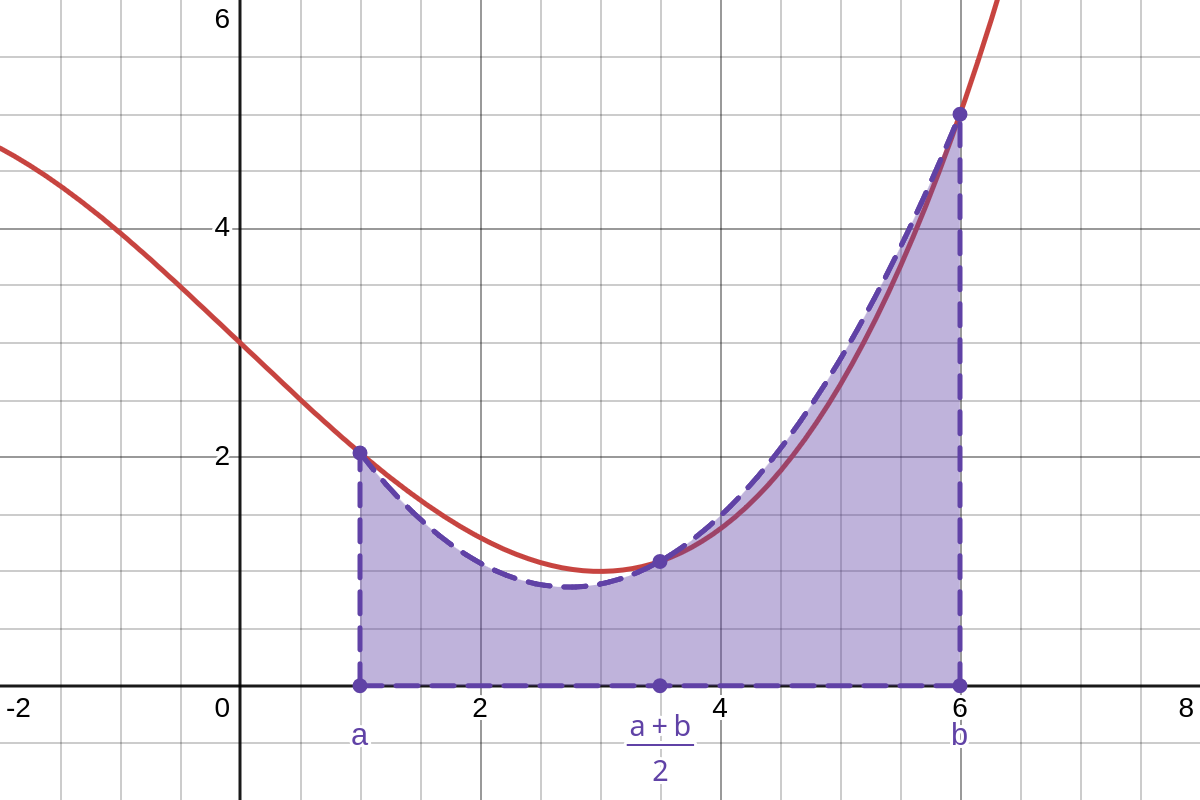
\includegraphics[scale=0.28]{../figures/simpson_cubic.png}
\end{center}

\subsubsection{Formula Gaussiana}

Rivediamo quindi il problema di massimizzare il grado di precisione dati i nodi $x_0, ..., x_n$.
Questo significherà imporre:
\[
	\begin{cases}
		E_n(1) = 0 \\
		E_n(x) = 0 \\
		\vdots \\
		E_n(x^{m + 1}) = 0
	\end{cases}
\]
cioè $m +1$ equazioni per $a_0, ..., a_m$, cioè $m + 1$ incognite.
Questo porta a:
\[
	\implies
	\begin{cases}
		m_0 = a_0 + a_1 + ... + a_n \\
		m_1 = a_0 x_0 + a_1 x_i + ... + a_n x_n \\
		\vdots \\
		m_n = a_0 x_0^n + a_1 x_1^n + ... + a_n x_n^n
	\end{cases}
\]
dove gli $m_i$ sono i risultati degli integrali dei monimoi $x^i$ sull'intervallo $[a, b]$ da cui:
$$
\implies
\begin{pmatrix}
	1 & 1 & ... & 1 \\
	x_0 & x_1 & ... & x_n \\
	x_0^2 & x_1^2 & ... & x_n^2 \\
	\vdots & \vdots & & \vdots \\
	x_0^n & x_1^n & ... & x_n^n
\end{pmatrix}
\begin{pmatrix}
	a_0 \\ \vdots \\ a_n
\end{pmatrix}
=
\begin{pmatrix}
	m_0 \\ \vdots \\ m_n
\end{pmatrix}
=
V^T
\begin{pmatrix}
	a_0 \\ \vdots \\ a_n
\end{pmatrix}
=
\begin{pmatrix}
	m_0 \\ \vdots \\ m_n
\end{pmatrix}
$$
Questo non è altro che un sistema lineare $(n + 1) \times (n + 1)$ con matrice di Vandermonde, da cui $\det(V) \neq 0$ e quindi se $x_i \neq x_j$ per ogni $i \neq j$, la soluzione del sistema è unica ed esiste un'unica formula di quadratura sui nodi $x_0, ..., x_n$ che ha grado di precisione $m \geq n$.

\par\smallskip

Potremmo considerare il problema diverso (e più difficile) di cercare sia i \textit{nodi} che i \textit{pesi} in modo da massimizzare il grado di precisione $m$.
In questo caso la formula di quadratura è sempre:
$$
J_n(f) = \sum_{i = 0}^n a_i f(x_i)
$$
e le incognite sono $2n + 2$, cioe gli $n + 1$ nodi $x_0, ..., x_n$ e gli $n + 1$ pesi $a_0, ..., a_n$.

Si impongono quindi $2n + 2$ equazioni del tipo:
\[
	\begin{cases}
		E_n(1) = 0 \\
		E_n(x) = 0 \\
		\vdots \\
		E_n(x^{2n + 1}) = 0
	\end{cases}
\]

L'unica cosa che sarà data sarà l'intervallo $[a, b]$ (non gli $x_i$), per cui otterremo un sistema non lineare:
\[
	\begin{cases}
		a_0 + a_1 + ... + a_n = m_0 \\
		a_0 x_0 + a_1 x_1 + ... + a_n x_n = m_1 \\
		\vdots \\
		a_0 x_0^{2n + 1} + a_1 x_1^{2n + 1} + ... + a_n x_n^{2n + 1} = m_{2n + 1}
	\end{cases}
\]

Fortunatamente esiste un teorema, che diamo senza dimostrazione:
\begin{theorem}{Unicità della formula Gaussiana}
	Il sistema:
\[
	\begin{cases}
		a_0 + a_1 + ... + a_n = m_0 \\
		a_0 x_0 + a_1 x_1 + ... + a_n x_n = m_1 \\
		\vdots \\
		a_0 x_0^{2n + 1} + a_1 x_1^{2n + 1} + ... + a_n x_n^{2n + 1} = m_{2n + 1}
	\end{cases}
\]
ammette sempre, dato $x_i \neq x_j$ per ogni $i \neq j$, un'unica soluzione per ogni scelta di $[a, b]$, $n$ e $\rho(x)$, con grado di precisione $\geq 2n + 1$.
\end{theorem}

Definiamo tale formula di quadratura come:
\begin{definition}{Formula Gaussiana}
	L'unica formula di quadratura su $[a, b]$ che verifica il sistema del teorema 16.1 (ovvero che massimizza il grado di precisione ottimizzando sia gli $x_i$ che gli $a_i$) si dice \textbf{formula Gaussiana} su $[a, b]$ con $n + 1$ nodi.
\end{definition}

Prendiamo ad esempio il caso $\rho = 1$, $n = 1$, e $[a, b] = [-1, 1]$ (analogamente a prima ma con i nodi liberi).
$$
\int_{-1}^1 f(x) \, dx \approx a_0 f(x_0) + a_1 f(x_1)
$$
con:
$$
a \leq x_0 < x_1 \leq b
$$

Imponiamo quindi:
\[
	\begin{cases}
		E_1(1) = 0 \\	
		E_1(x) = 0 \\	
		E_1(x^2) = 0 \\	
		E_1(x^3) = 0 \\	
	\end{cases}
	\rightarrow
	\begin{cases}
		a_0 + a_1 = 2 \\
		a_0 x_0 + a_1 x_1 = 0 \\
		a_0 x_0^2 + a_1 x_1^2 = \frac{2}{3} \\
		a_0 x_0^3 + a_1 x_1^3 = 0
	\end{cases}
\]
per risolvere il sistema ricaviamo prima $a_0$ e $a_1$ in funzione di $x_0$ e $x_1$ dalle prime 2 equazioni:
\begin{itemize}
	\item $a_0$ si ha direttamente dalla prima equazione:
		$$
			a_0 = 2 - a_1
		$$
	\item $a_1$ si ha dalla seconda equazione,, sostituendo la formula per $a_0$ appena trovata:
		$$
		(2 - a_1) x_0 + a_1 x_1 = 2x_0 - a_1 x_0 + a_1 x_1 = 0 \implies a_1 (x_1 - x_0) = \frac{-2 x_0}{x_1 - x_0}
		$$
\end{itemize}
da cui abbiamo che vale:
$$
a_0 = \frac{2 x_1}{x_1 - x_0}, \quad a_1 = -\frac{2 x_0}{x_1 - x_0}
$$
Prendiamo quindi il sistema ridotto alle ultime 2 equazioni:
\[
	\begin{cases}
		\frac{2 x_1 x_0^2}{x_1 - x_0} - \frac{2 x_0 x_1^2}{x_1 - x_0} = \frac{2}{3} \\ 
		\frac{2 x_1 x_0^3}{x_1 - x_0} - \frac{2 x_0 x_1^3}{x_1 - x_0} = 0
	\end{cases}
	\rightarrow 
	\begin{cases}
		2 x_1 x_0^2 - 2 x_0 x_1^2 = \frac{2}{3} (x_1 - x_0) \\ 
		2 x_1 x_0^3 - 2 x_0 x_1^3 = 0
	\end{cases}
\]
dall'ultima di queste si ricava:
$$
2 x_1 x_0^3 - 2 x_0 x_1^3 = 0 \, \Rightarrow \, 2 x_1 x_0^3 = 2 x_0 x_1^3 \, \Rightarrow \, x_0^2 = x_1^2 \, \Rightarrow \, x_0 = \pm x_1
$$
Ci interesserà prendere $x_0 = - x_1$, da cui dalla prima equazione:
$$
2 x_1^3 + 2 x_1^4 = \frac{4}{3} x_1 \implies x_1^2 = \frac{1}{3}
$$
cioè:
$$
x_0, x_1 = \pm \frac{\sqrt{3}}{3}
$$
sostituendo nelle formule per $a_0$ e $a_1$ trovate prima, si ha poi immediatamente:
$$
a_0, a_1 = 1, \quad 
$$
cioè la formula Gaussiana è:
$$
J_1(f) = f\left(-\frac{\sqrt{3}}{3}\right) + f\left(\frac{\sqrt{3}}{3}\right)
$$
che vale fino al grado 3, in quanto al grado 4 si ha:
$$
E_1(x^4) = \frac{2}{5} - \frac{2}{9} \neq 0
$$
da cui il grado di precisione è esattamente 3. \qed

\subsubsection{Errore nelle formule di quadratura}
Riguardo all'errore già definito nella definizione 16.2, vale il seguente teorema:
\begin{theorem}{Teorema di Peano}
	Data una funzione $f(x) \in \mathbb{C}^{n + 1} \left([a, b]\right)$, cioè derivabile $n+1$ volte, con $m$ grado di precisione della formula di quadratura $J_n$, allora l'errore $E_n$ (vedi definizione 16.2) si può scrivere come:
	$$
		E_n(f) = I(\rho, f) - J_n(f) = \frac{1}{m!} \int_a^b f^{(m + 1)}(t) \cdot G(t) \, dt
	$$
	dove la $G(t)$ è:
	$$
		G(t) = E_n (s_m (x - t)) = I(\rho \cdot s_m(x - t)) - J_n (s_m(x - t))
	$$
	e la $s_m(x)$ è:
	$$
		s_m(x) = 
		\begin{cases}
			x^m, \quad x \geq 0 \\
			0, \quad x < 0
		\end{cases}
	$$
	cioè la $s_m(x - t)$ non è altro che la $s_m(x)$ spostata a destra di $t$.
\end{theorem}
Vale la definizione:
\begin{definition}{Nucleo di Peano}
	La funzione $G(t)$ del teorema 16.2 è detta \textbf{nucleo di Peano}. 
\end{definition}

\end{document}
